%=============================================================================
%  report_ieee14_all_gfm_constraints_en.tex
%  English report: why the four IEEE-14 converters are NOT all switched to
%  grid-forming, argued from the underlying CONSTRAINTS, led by the
%  short-circuit-ratio (SCR) screen.
%
%  Answers one question, in this order:
%    Q  why is the forming set not pinned to all four, and what exactly is
%       wrong if it is?
%    A  (1) the SCR screen -- what it measures, why the count cannot move it,
%           and what a weak grid does to a PLL converter;
%       (2) the constraint stack behind the decision, each gate reported by
%           name and none tradeable against another;
%       (3) what "switching all four" actually costs -- measured outcomes.
%
%  EVIDENCE BASE
%  - Every measured number is read out of a named artefact of the delivered
%    result set (output/diagnostics/ieee14_gfm_lock_compare_zeta/, built by
%    scripts/reporting/run_ieee14_gfm_lock_comparison.m), out of a generated
%    table under docs/source/figures/, or out of a named source line of the
%    production code. Nothing is interpolated, estimated or re-tuned.
%  - Where a quantity is a published diagnostic rather than an active gate,
%    it is labelled as such at the point of use.
%  - The caches themselves are not in this worktree (they are gitignored
%    build outputs). The numbers reproduced here are the ones already
%    carried by the delivered report artefacts of the same result set, and
%    each is attributed to its own file so it can be re-derived.
%
%  BUILD:  xelatex report_ieee14_all_gfm_constraints_en.tex   (twice)
%=============================================================================
\documentclass[12pt,a4paper]{article}

\usepackage{graphicx,amsmath,amssymb,float,caption,hyperref,fancyhdr}
\usepackage{amsthm}
\usepackage{newtxtext,newtxmath}
\newtheorem{proposition}{Proposition}
\theoremstyle{remark}
\newtheorem{remark}{Remark}
\usepackage{geometry,booktabs,tabularx,array,longtable,microtype}
\usepackage{xcolor}
\usepackage{enumitem}
\usepackage{tikz}
\usetikzlibrary{arrows.meta,positioning,calc,patterns,shapes.geometric}
\geometry{margin=1in}
\setlength{\headheight}{14.5pt}
\pagestyle{fancy}
\fancyhf{}
\lhead{IEEE-14: why not all four converters form}
\rhead{\thepage}
\renewcommand{\headrulewidth}{0.4pt}
\renewcommand{\arraystretch}{1.14}
\emergencystretch=3em
\sloppy

\definecolor{navy}{RGB}{25,55,95}
\definecolor{ok}{RGB}{0,110,70}
\definecolor{no}{RGB}{170,40,35}
\definecolor{warn}{RGB}{175,110,0}
\definecolor{pale}{RGB}{240,244,249}

\newcommand{\pu}{\,\mathrm{pu}}
\newcommand{\Ibr}{\mathrm{IBR}}
\newcommand{\zmin}{\zeta_{\min}}
\newcommand{\zworst}{\zeta_{\mathrm{worst}}}
\newcommand{\greq}{\gamma_{\mathrm{req}}}
\newcommand{\Ssev}{S}
% Code identifiers: monospaced with hyphenation disabled, so a long identifier is
% never hyphenated mid-word (which for names like `eligible_for_scr` reads as a
% typo). Line breaking is instead absorbed by the stretch settings below.
\newcommand{\code}[1]{{\ttfamily\small\hyphenchar\font=-1 #1}}
\newcommand{\measured}{\textcolor{ok}{\textbf{[measured]}}}
\newcommand{\derived}{\textcolor{warn}{\textbf{[derived]}}}
\newcommand{\sourcecode}{\textcolor{navy}{\textbf{[source]}}}

\title{\bfseries Why the IEEE-14 converters are not all switched to grid-forming\\[4pt]
\large The short-circuit-ratio screen and the constraint stack behind the count}
\author{In-house power system analysis toolkit}
\date{}

\begin{document}
\maketitle
\thispagestyle{fancy}

\begin{abstract}
\noindent
The IEEE-14 study network carries one synchronous machine at bus~1 and four
dual-mode converters at buses 2, 3, 6 and 8. When the machine trips, the
supervisor promotes converters to grid-forming (GFM) one or two at a time, and
never pins all four for the islanded window. This report answers why, and it
leads with the short-circuit ratio.

Three results carry the argument. First, \textbf{the SCR of this island is below
the WECC strong-grid floor of $3$ on $98.61\%$ of all converter-samples, and on
$100\%$ of the islanded window}, whose mean is $2.3015$ --- yet \emph{promoting a
converter cannot raise it}, because the Thevenin impedance in the definition is
built from branch data, bus shunts and reference grounding alone and contains no
term for the forming count. SCR is a constraint on the \emph{plant}, not a lever
the supervisor can pull. Second, \textbf{the count is bounded from both sides by
constraints the supervisor cannot trade}: with no former the island is refused
outright at $t=20.0000$\,s with \code{noVoltageFormingSource}, and with all four
pinned it dies at $25.4852$\,s --- $5.49$\,s after the trip, before the load
step and before any fault. Third, \textbf{the intervening sets are not all
available}: of the fifteen non-empty forming sets, only seven are admissible,
\emph{every} three-converter set has no equilibrium at all, and the all-four set
--- although admissible --- is the least damped of the seven
($\zworst = 0.1223$ against $0.2549$--$0.2676$, less than half). The conclusion
this report defends is not ``fewer formers are better'': it is that
\textbf{the forming count is not a free parameter, stability is not monotone in
it, and the SCR screen explains why adding converters does not buy the strength
that is missing}.
\end{abstract}

\tableofcontents
\clearpage

%=============================================================================
\section{The question, and the shape of the answer}
%=============================================================================

\subsection{What is being asked}

Four converters sit at buses 2, 3, 6 and 8, each able to run grid-following
(GFL) or grid-forming (GFM). One machine at bus~1 owns the angle reference. When
it trips at $t=20$\,s, at least one converter must own the reference or the
island has no defined voltage angle. The natural engineering reflex is to make
\emph{all four} form the grid: maximum voltage support, maximum inertia, no
follower left depending on a reference that no longer exists.

The delivered supervisor does not do that. Its forming set across the islanded
window takes the values

\begin{equation}
1 \;\to\; 2 \;\to\; 1 \;\to\; 2 \;\to\; 4 \;\to\; 1 \;\to\; 2 \;\to\; 1,
\label{eq:countseq}
\end{equation}

with durations $36.98$\,s, $9.37$\,s and $92.90$\,s at one, two and four
formers respectively, and it never performs a one-step jump from one former
straight to four. \measured{} \code{report\_ieee14\_switching\_decision\_basis\_en}, \S7.

The question is therefore precise: \emph{why is the count chosen, rather than
maximised, and what is actually wrong with switching all four?}

\subsection{The answer in one paragraph}

Because the quantity that is actually deficient on this island --- short-circuit
strength --- is a property of the \emph{network}, and the forming count is not a
term in it. Adding formers cannot repair a weak grid; it changes a different
question, from ``can the followers lock to a stiff bus?'' to ``can four voltage
sources share current on a network whose impedance none of them can change?''.
This network answers that second question badly. Measured: all four
three-converter sharings have no equilibrium at all, and the four-converter
sharing is admissible but the least damped of the seven admissible sets. So the
count is set by the constraint stack --- equilibrium existence, device limits,
full-KCL small-signal margin, reference ownership and the transition
certificate --- and those constraints are non-tradeable, meaning a comfortable
margin on one does not buy a pass on another.

\subsection{Roadmap}

Section~\ref{sec:scr} treats the SCR screen in detail: the definition, the
source line that forces its applicability policy, the delivered measurements, and
four consequences that follow from it. Section~\ref{sec:constraints} lays out the
constraint stack and shows, gate by gate, what refuses \emph{all four}.
Section~\ref{sec:cost} measures what pinning all four actually costs.
Section~\ref{sec:notclaimed} states the limits of the claim.

%=============================================================================
\section{The short-circuit-ratio screen}\label{sec:scr}
%=============================================================================

\subsection{Definition, exactly as implemented}

For each online converter the project computes
(\code{+stability/ibr\_scr\_metrics.m}, header at \code{:29--49})

\begin{equation}
\mathrm{SCR}_i \;=\; \frac{S_{sc,i}}{S_{\mathrm{rated},i}},
\qquad
S_{sc,i} \;=\; \frac{|V_i|^2}{|Z_{th,ii}|}\,S_{\text{base}},
\qquad
Z_{th,ii} \;=\; \bigl[\,\mathbf{Y}^{-1}\mathbf{e}_i\,\bigr]_i ,
\label{eq:scr}
\end{equation}

solved as \code{Ybus * Vz = e\_k} and read at \code{Vz(k)} --- the source
comment states explicitly that this is ``\emph{never} \code{inv}/\code{pinv}''
\sourcecode. The matrix $\mathbf{Y}$ is built from branch data including tap and
phase shift, plus bus shunts, and from nothing else:

\begin{quote}\small
\code{No load admittance - pure network strength (PROJECT\_DERIVED choice).}
\code{\hfill(ibr\_scr\_metrics.m:26)}
\end{quote}

Reference buses are grounded so that the Thevenin equivalent is taken with the
voltage sources short-circuited. The rating is the converter's own
\code{ratings.Mbase}; if it is missing or non-positive the evaluation
\emph{fails closed} rather than inferring one, and the header records that
\code{ratings.Sbase} and \code{limits.Pmax\_MW} are deliberately \emph{not}
accepted as fallbacks \sourcecode.

The threshold and its polarity are fixed:

\begin{equation}
\text{pass} \;=\; \mathrm{SCR} > 3,
\qquad
\text{refuse} \;=\; \mathrm{SCR} \le 3,
\label{eq:threshold}
\end{equation}

classified \code{CASE\_DEFINED} and described in the source as the
``\emph{WECC REGC\_A strong-grid contract}'' \sourcecode{} --- that is, the
screen a transmission planner applies before allowing a \emph{grid-following}
plant to connect.

\subsection{The property that decides the whole argument}

Equation~\eqref{eq:scr} contains no term for control mode. $\mathbf{Y}$ is
branch data, bus shunts and reference grounding; $S_{\mathrm{rated},i}$ is a
nameplate number; $|V_i|$ is a measurement. Therefore:

\begin{quote}
\textbf{Promoting a converter from GFL to GFM cannot change $Z_{th}$, and cannot
change $S_{\mathrm{rated}}$. The forming count does not enter
\eqref{eq:scr} at all.}
\end{quote}

This is not a numerical accident of one run; it is a property of the equation
\sourcecode. It is the single most important fact in this report, because it
means the intuition ``the grid is weak, therefore form more converters'' cannot
be executed through SCR. SCR can move only through the measured numerator
$|V_i|^2$ --- that is, only as a \emph{consequence} of the island's behaviour,
never as a \emph{lever} the supervisor pulls.

\begin{remark}[Scope that must travel with the number]
In \code{ibr\_scr\_metrics.m:301--307} the screening profile is forced to
\code{'not\_applicable\_full\_state\_source\_model'} for the project's
full-state dual family (\code{model\_id} $=$ \code{'eecon49\_dual'}), and the
source comment explains why: this family ``\emph{models the plant explicitly, so
the WECC strong-grid SCR screening profile does not apply to it}''. The
consequence is \code{eligible\_for\_scr = false} with \code{pass = true} and the
recorded reason ``\emph{SCR threshold not applicable to this full-state model;
equilibrium, limits and full-KCL SSSA remain mandatory}''. On the delivered case
all four converters report \code{eligible\_for\_scr = 0}, \code{SCR = NaN},
\code{pass = 1}. \measured

The SCR figures quoted below are therefore a \textbf{published per-sample
diagnostic, not an active gate}. That does not weaken the argument: the
network-invariance of \eqref{eq:scr} is a property of the equation, and holds
whether or not the gate is armed. It does mean the number must not be presented
as a pass/fail verdict of this run.
\end{remark}

\subsection{The delivered measurements}

\begin{table}[H]
\centering
\small
\begin{tabular}{@{}lrrrrr@{}}
\toprule
\textbf{Window} & $n$ & \textbf{min} & \textbf{mean} & \textbf{max} & \textbf{below 3}\\
\midrule
pre-trip, machine online & $168$ & $2.0892$ & $2.3439$ & $2.4803$ & $100.00\%$\\
post-trip, islanded      & $2760$ & $0.6501$ & $\mathbf{2.3015}$ & $2.8147$ & $\mathbf{100.00\%}$\\
after the load step      & $3152$ & $1.5411$ & $2.6899$ & $3.2908$ & $95.53\%$\\
fault at bus 9, $85.00$--$85.15$ & $164$ & $0.2944$ & $1.2954$ & $6.6726$ & $97.56\%$\\
line 6--13 out           & $2160$ & $2.0718$ & $2.7319$ & $6.6184$ & $97.96\%$\\
restore to reclose       & $4384$ & $1.8361$ & $2.5914$ & $3.5322$ & $99.64\%$\\
after reclose            & $1928$ & $1.9104$ & $2.3291$ & $2.4833$ & $100.00\%$\\
\midrule
whole run, all four converters & $14716$ & $0.2944$ & $2.5271$ & $6.6726$ & $\mathbf{98.61\%}$\\
\bottomrule
\end{tabular}
\caption{Per-sample SCR at the converter buses. Reproduced from
\code{report\_ieee14\_switching\_decision\_basis\_en}, Table~7, which reads it
from the run's own \code{agsi\_reference.scr} diagnostic; classification
\code{ASSUMED\_DIAGNOSTIC}. The ratio uses each converter's rated MVA on the
system base ($100$\,MVA), and the numerator uses the measured bus voltage of
that sample. \measured}
\label{tab:scr}
\end{table}

\begin{figure}[H]
\centering
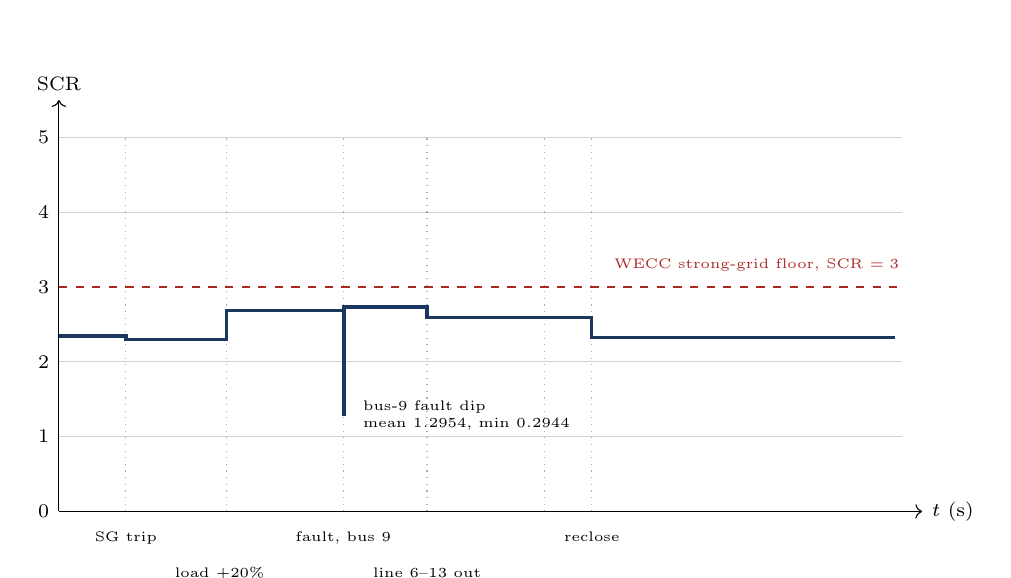
\begin{tikzpicture}[font=\scriptsize,x=0.0425cm,y=0.95cm]
\foreach \y in {1,2,4,5} \draw[gray!35] (0,\y)--(252,\y);
\draw[no,thick,dashed] (0,3)--(252,3);
\foreach \y in {0,1,2,3,4,5} \node[left,font=\scriptsize] at (0,\y) {\y};
\draw[->] (0,0)--(258,0) node[right,font=\scriptsize]{$t$ (s)};
\draw[->] (0,0)--(0,5.5) node[above,font=\scriptsize]{SCR};
\foreach \x in {20,50,85,110,145,159.25}
  \draw[gray!65,dotted] (\x,0)--(\x,5);
\draw[navy,very thick]
  (0,2.3439)--(20,2.3439)--(20,2.3015)--(50,2.3015)--(50,2.6899)
  --(85,2.6899)--(85,1.2954)--(85.15,1.2954)--(85.15,2.7319)
  --(110,2.7319)--(110,2.5914)--(159.25,2.5914)
  --(159.25,2.3291)--(250,2.3291);
\node[no,anchor=south west,font=\tiny] at (163,3.08)
  {WECC strong-grid floor, SCR $=3$};
\node[anchor=west,font=\tiny,align=left] at (88,1.28)
  {bus-9 fault dip\\mean $1.2954$, min $0.2944$};
\node[anchor=north,font=\tiny] at (20,-0.14) {SG trip};
\node[anchor=north,font=\tiny] at (85,-0.14) {fault, bus 9};
\node[anchor=north,font=\tiny] at (159.25,-0.14) {reclose};
\node[anchor=north,font=\tiny] at (48,-0.62) {load $+20\%$};
\node[anchor=north,font=\tiny] at (110,-0.62) {line 6--13 out};
\end{tikzpicture}
\caption{The mean SCR across the four converters, drawn as a step plot of the
per-window means of Table~\ref{tab:scr}. The dashed line is the WECC strong-grid
floor. \textbf{The island never leaves the weak-grid region, in any window, at
any time.}}
\label{fig:scrplot}
\end{figure}

\subsection{Four consequences}

\begin{enumerate}[leftmargin=1.7em,itemsep=3pt]
\item \textbf{The machine trip barely moves SCR --- and that is the point, not
      an error.} The window mean goes $2.3439 \to 2.3015$. $Z_{th}$ is built
      from the passive network, and the machine is not a term in it. What changes
      at the trip is the numerator and, decisively, \emph{which sources are
      behind the bus}: before the trip the converters are followers on a network
      held up by a $615$\,MVA machine; after it they are the only sources on the
      same network. \textbf{The impedance seen is the same; the support behind it
      is not.} That is precisely the condition grid-forming control exists to
      address --- and precisely why the answer is ``at least one must form''
      rather than ``four must form''.

\item \textbf{The island is weak by the WECC definition essentially always.}
      $98.61\%$ of the delivered run's converter-samples sit at or below the
      floor that REGC\_A uses to \emph{refuse} a grid-following plant. The
      post-trip window and the post-reclose window are each $100\%$ below it, and
      no window's mean reaches it. The deepest value, $0.2944$, occurs during the
      fault, where a collapsed bus voltage is the whole of the numerator.
      \measured

\item \textbf{Because the count cannot move \eqref{eq:scr}, pinning all four
      does not fix the weak grid.} It leaves the weakness in place and adds three
      more voltage sources that must now share current against the same
      unchanged, high network impedance. The problem changes \emph{kind}: the
      REGC\_A screen asks whether a PLL can lock to a stiff bus, and with all
      four forming there is no PLL left to protect. The screening question
      becomes vacuous, and is replaced by a different and harder one ---
      multi-source current sharing on a weak network --- which
      Section~\ref{sec:constraints} shows this network answers badly.
      \derived{} from \eqref{eq:scr} and \sourcecode.

\item \textbf{The load step \emph{raises} SCR, which warns against cross-window
      comparison.} The window mean rises $2.3015 \to 2.6899$ after the $+20\%$
      step: load admittance is excluded from $\mathbf{Y}$, but load current
      raises bus voltage, and $|V|^2$ is the numerator. As implemented,
      \eqref{eq:scr} is a \emph{voltage-referenced} quantity, not a pure network
      invariant. Comparisons are valid \emph{within} a row of
      Table~\ref{tab:scr}, not across rows.
\end{enumerate}

\begin{remark}[A rating-convention caveat, so the number is not over-read]
A second diagnostic in the repository
(\code{build\_ieee14\_switch\_system.m:159}) computes the same $|V|^2/|Z_{th}|$
but divides by $\max(|S_{\text{bus}}|,0.20)$ rather than by the converter
rating, and reports $4.78$--$7.19$ for the same four buses with the machine
online. \textbf{Same impedance, different denominator.} The numbers in
Table~\ref{tab:scr} are the ones the running supervisor's own diagnostic
produces, on the rated-MVA convention, and the conclusions drawn above are
conclusions about the \emph{impedance} and the \emph{count}, both of which are
convention-independent.
\end{remark}

%=============================================================================
\section{The constraint stack behind the count}\label{sec:constraints}
%=============================================================================

The supervisor is three stages in series and \textbf{each stage can only
refuse} --- no stage may overrule another's refusal, and no gate is traded
against another inside a scalar. The project states this as a standing rule:

\begin{quote}\small\itshape
``Short-circuit strength, device current limits, and reference ownership are
separate non-tradeable gates, never traded off against each other inside one
scalar.''\par
\raggedleft\normalfont\code{(README.md:84--86)}\par
\end{quote}

That sentence is the reason the answer to ``why not all four?'' is a
\emph{stack} of independent refusals rather than a single score.

\subsection{Constraint 1 --- a voltage-forming source must exist}

With all four locked in grid-following, the machine is the only voltage-forming
source, so opening its breaker leaves an energised island with \emph{no angle
reference}. The per-island admissibility check refuses the transaction
\emph{before any Newton solve}: the delivered \code{locked\_gfl} arm ends at
$t=20.0000$\,s after $43$ samples with the identifier
\code{noVoltageFormingSource}. \measured

\begin{quote}
On this resource mix, promoting \textbf{at least one} converter to grid-forming
is therefore a \emph{necessary condition} for a post-trip trajectory to exist at
all --- not an improvement to one.
\end{quote}

This is the hard \emph{lower} bound on the count, and it is measured, not
argued.

\subsection{Constraint 2 --- an equilibrium must exist}

There are $2^4-1 = 15$ non-empty forming sets. The project solves every one at
its own operating point before the run starts.

\begin{table}[H]
\centering
\small
\begin{tabular}{@{}clrrcl@{}}
\toprule
\textbf{Set} & \textbf{Ref} & $\omega$ (rad/s) & $\mathrm{margin}$ & $\zworst$ & \textbf{Outcome}\\
\midrule
$\{5\}$        & 5 & $-0.155437$ & $+0.055437$ & $0.2676$ & admissible\\
$\{4\}$        & 4 & $-0.252025$ & $+0.152025$ & $0.2629$ & admissible\\
$\{3\}$        & 3 & $-0.316711$ & $+0.216711$ & $0.2618$ & admissible\\
$\{2\}$        & 2 & $-0.328014$ & $+0.228014$ & $0.2569$ & admissible\\
$\{2,4\}$      & 2 & $-0.561723$ & $+0.461723$ & $0.2549$ & admissible\\
$\{3,4\}$      & 3 & $\mathbf{-0.568138}$ & $\mathbf{+0.468138}$ & $0.2560$ & admissible (most damped)\\
\midrule
$\{2,3\}$      & --- & --- & --- & --- & no equilibrium: IBR6 violates a limit\\
$\{2,5\}$      & --- & --- & --- & --- & no equilibrium: IBR6 violates a limit\\
$\{3,5\}$      & --- & --- & --- & --- & no equilibrium: IBR6 violates a limit\\
$\{4,5\}$      & --- & --- & --- & --- & no equilibrium: IBR3 violates a limit\\
\midrule
$\{2,3,4\}$    & --- & --- & --- & --- & no equilibrium, residual $3.279\times10^{2}$\\
$\{2,3,5\}$    & --- & --- & --- & --- & no equilibrium, residual $3.605\times10^{2}$\\
$\{2,4,5\}$    & --- & --- & --- & --- & no equilibrium, residual $3.561\times10^{2}$\\
$\{3,4,5\}$    & --- & --- & --- & --- & no equilibrium, residual $3.346\times10^{2}$\\
\midrule
$\{2,3,4,5\}$  & 2 & $-0.482909$ & $+0.382909$ & $\mathbf{0.1223}$ & admissible, \textcolor{no}{\textbf{least damped}}\\
\bottomrule
\end{tabular}
\caption{The complete SG-off admissibility enumeration, read from
\code{summary.shared.sg\_off\_candidates} in
\code{ieee14\_gfm\_lock\_compare\_zeta/summary.mat} and reproduced from
\code{report\_ieee14\_switching\_decision\_basis\_en}, Table~4. Seven of fifteen
sets are admissible. $\omega$ is the least damped member of the frozen
finite-difference set; $\mathrm{margin} = -\omega - \greq$; $\zworst$ is the
worst damping ratio over the physical decision spectrum. This is a
\emph{base-load table, frozen before candidate evaluation}. \measured}
\label{tab:adm}
\end{table}

\begin{figure}[H]
\centering
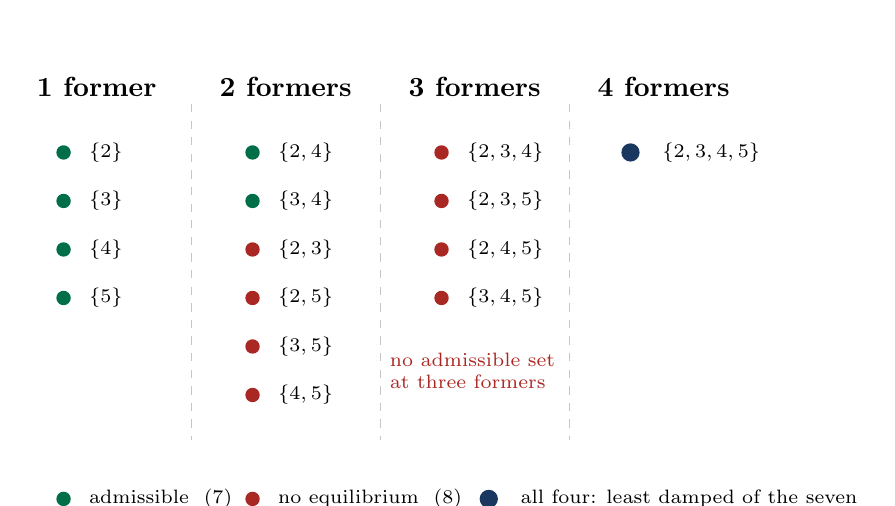
\begin{tikzpicture}[font=\scriptsize,x=1cm,y=0.88cm]
\node[font=\bfseries] at (0.42,0.95) {1 former};
\node[font=\bfseries] at (2.82,0.95) {2 formers};
\node[font=\bfseries] at (5.22,0.95) {3 formers};
\node[font=\bfseries] at (7.62,0.95) {4 formers};
\foreach \x in {1.62,4.02,6.42} \draw[gray!45,dashed] (\x,0.7)--(\x,-4.15);
\fill[ok] (0,0) circle (2.6pt);      \node[anchor=west] at (0.2,0)      {$\{2\}$};
\fill[ok] (0,-0.7) circle (2.6pt);   \node[anchor=west] at (0.2,-0.7)   {$\{3\}$};
\fill[ok] (0,-1.4) circle (2.6pt);   \node[anchor=west] at (0.2,-1.4)   {$\{4\}$};
\fill[ok] (0,-2.1) circle (2.6pt);   \node[anchor=west] at (0.2,-2.1)   {$\{5\}$};
\fill[ok] (2.4,0) circle (2.6pt);    \node[anchor=west] at (2.6,0)      {$\{2,4\}$};
\fill[ok] (2.4,-0.7) circle (2.6pt); \node[anchor=west] at (2.6,-0.7)   {$\{3,4\}$};
\fill[no] (2.4,-1.4) circle (2.6pt); \node[anchor=west] at (2.6,-1.4)   {$\{2,3\}$};
\fill[no] (2.4,-2.1) circle (2.6pt); \node[anchor=west] at (2.6,-2.1)   {$\{2,5\}$};
\fill[no] (2.4,-2.8) circle (2.6pt); \node[anchor=west] at (2.6,-2.8)   {$\{3,5\}$};
\fill[no] (2.4,-3.5) circle (2.6pt); \node[anchor=west] at (2.6,-3.5)   {$\{4,5\}$};
\fill[no] (4.8,0) circle (2.6pt);    \node[anchor=west] at (5.0,0)      {$\{2,3,4\}$};
\fill[no] (4.8,-0.7) circle (2.6pt); \node[anchor=west] at (5.0,-0.7)   {$\{2,3,5\}$};
\fill[no] (4.8,-1.4) circle (2.6pt); \node[anchor=west] at (5.0,-1.4)   {$\{2,4,5\}$};
\fill[no] (4.8,-2.1) circle (2.6pt); \node[anchor=west] at (5.0,-2.1)   {$\{3,4,5\}$};
\fill[navy] (7.2,0) circle (3.3pt);  \node[anchor=west] at (7.48,0)     {$\{2,3,4,5\}$};
\node[anchor=north west,align=left,text=no] at (4.02,-2.75)
  {no admissible set\\at three formers};
\fill[ok] (0,-5.0) circle (2.6pt);
\node[anchor=west] at (0.2,-5.0) {admissible \ (7)};
\fill[no] (2.4,-5.0) circle (2.6pt);
\node[anchor=west] at (2.6,-5.0) {no equilibrium \ (8)};
\fill[navy] (5.4,-5.0) circle (3.3pt);
\node[anchor=west] at (5.68,-5.0) {all four: least damped of the seven};
\end{tikzpicture}
\caption{The admissibility map. \textbf{Feasibility is not monotone in the
number of forming converters}: every admissible set sits below or above the
three-unit row, never on it. Going from two units to three is not a compromise
--- it lands where the equations have no solution at all.}
\label{fig:map}
\end{figure}

Three facts here are load-bearing.

\begin{enumerate}[leftmargin=1.7em,itemsep=3pt]
\item \textbf{Eight of fifteen sets do not exist as operating points.} Four
      fail because a converter left in grid-following is asked to violate an
      operating limit; four fail because the four-way power balance has no
      solution at all (coupled-Newton residuals $3.28$--$3.61\times10^{2}$).
      Each failure is \emph{reported by name}, not as a low margin.
\item \textbf{All four three-converter sets fail.} The middle of the map is
      empty at every one of the four ways of choosing three. A policy that
      climbed the count one at a time would be refused at the third step.
\item \textbf{The all-four set is admissible but is the outlier.} Its worst
      damping ratio, $0.1223$, is \emph{less than half} of every other
      admissible set's $0.2549$--$0.2676$, and it is the only admissible set
      whose worst ratio is not comfortably above the floor. It passes the gate
      --- and is the worst of the seven that pass.
\end{enumerate}

\subsection{Constraint 3 --- the damping-ratio floor, at three perturbation
sizes}

The acceptance criterion is declared by the case, not chosen by this report:
\code{acceptance\_criterion} $=$ \code{'damping\_ratio\_floor'}, with
\code{zeta\_min\_damping} $= 0.05$ and
\code{frozen\_before\_candidate\_eval} $= 1$ \sourcecode. A candidate is
admissible only when

\begin{equation}
\forall \varepsilon \in \{1.5,\,3,\,6\}\times10^{-6}:\quad
\max\operatorname{Re}\lambda(\varepsilon) < 0
\quad\text{and}\quad
\min_i \zeta_i(\varepsilon) \;\ge\; 0.05,
\qquad
\zeta_i = \frac{-\operatorname{Re}\lambda_i}{|\lambda_i|}.
\label{eq:gate}
\end{equation}

Three features of \eqref{eq:gate} matter for the count question.

\begin{itemize}[leftmargin=1.5em,itemsep=2pt]
\item \textbf{It is a floor on the \emph{worst} mode, not on the rightmost.}
      The worst-damped mode is generally not the rightmost one, so reading the
      margin off $\max\operatorname{Re}\lambda$ would miss it.
\item \textbf{It is a \emph{ratio}, so it is timescale-invariant.} This plant
      carries modes from roughly $0.02$\,Hz --- the island's electromechanical
      swing, slowed by the converters' small inertia --- up to the current-loop
      band, a span of more than three decades. No single absolute decay rate is
      a meaningful floor across that span; a ratio is.
\item \textbf{All three perturbation sizes must agree.} Disagreement fails
      closed. A margin that exists at one finite-difference step but not at the
      next is not a margin.
\end{itemize}

The separate quantity $\greq = 0.1$\,rad/s is the \emph{ordering key} among
already-admissible candidates only --- it is not the gate. This is why a set can
be admissible while its \code{margin} is negative, as IBR8's is at
$\mathrm{margin} = +0.055437$ against a gate that never consults it.

\subsection{Constraint 4 --- the count is chosen as a minimum, not a maximum}

The runtime rule is the following, and it is the direct answer to the count
question.

\begin{proposition}[Minimum-cardinality admissible superset]
\label{prop:superset}
Let $\mathcal{F}$ be the forming set at the decision instant and $\mathcal{T}$
the set of table rows with \code{feasible} and \code{ready\_to\_commit} both
true. The returned destination is the row $c \in \mathcal{T}$ minimising, in
order: (i) $|\mathrm{selected}(c)|$; (ii) $-\mathrm{margin}(c)$; (iii) the
selected index tuple lexicographically; (iv) the reference index --- subject to
$\mathcal{F} \subsetneq \mathrm{selected}(c)$, i.e.\ the destination must be a
\emph{strict} superset of the current set
\code{(select\_support\_augmentation\_candidate.m:54--58, 101--112)}. If no such
row exists the function returns \code{found=false} and the supervisor holds its
incumbent set; it never fabricates a candidate and never relaxes a gate.
\end{proposition}

Two consequences follow immediately. \textbf{The cardinality objective is a
minimum}: nothing in Proposition~\ref{prop:superset} rewards adding converters,
and a three-unit destination is chosen over a two-unit one \emph{only} when no
two-unit strict superset is admissible. And \textbf{the choice is not a free
re-selection}: because the destination must contain the current set, the
supervisor cannot answer ``the island needs four formers'' by promoting four at
once from one; it can only add to what it has, and it adds as few as the table
permits. On the delivered chronology the resolution is

\begin{table}[H]
\centering
\small
\begin{tabularx}{\textwidth}{@{}r l X l l@{}}
\toprule
$t$ (s) & \textbf{incumbent $\mathcal{F}$} & \textbf{candidate supersets} & \textbf{admissible} & \textbf{chosen}\\
\midrule
$22.0887$ & $\{2\}$ & all seven supersets of $\{2\}$
          & $\{2,4\}$, $\{2,3,4,5\}$ & $\{2,4\}$\\
$51.3403$ & $\{2\}$ & (as above) & $\{2,4\}$, $\{2,3,4,5\}$ & $\{2,4\}$\\
$53.3795$ & $\{2,4\}$ & $\{2,3,4\}$, $\{2,4,5\}$, $\{2,3,4,5\}$ & $\{2,3,4,5\}$ only & $\{2,3,4,5\}$\\
$148.2811$& $\{2\}$ & (as at $22.0887$) & $\{2,4\}$, $\{2,3,4,5\}$ & $\{2,4\}$\\
\bottomrule
\end{tabularx}
\caption{Every augment of the delivered chronology resolved through
Proposition~\ref{prop:superset} using the admissibility of
Table~\ref{tab:adm}. \measured}
\label{tab:resolution}
\end{table}

At $t=22.0887$\,s and $t=51.3403$\,s two destinations exist and the smaller one
wins on criterion~(i). At $t=53.3795$\,s --- after the $+20\%$ load step, with
the island carrying the machine's $133.19$\,MW deficit --- the two-unit supersets
$\{2,3,4\}$ and $\{2,4,5\}$ are among the eight rows with no equilibrium, so the
only admissible destination is the all-four set and criterion~(i) has nothing to
choose. \textbf{Four forming converters is not a policy preference; it is the
residue of the enumeration after the load step.}

\begin{quote}\small\itshape
The four-unit promotion happens because at $+20\%$ load nothing smaller can be
certified --- not because four was judged better than two.
\end{quote}

\subsection{Constraint 5 --- the transition, not just the destination}

Stage~3 re-simulates the would-be committed state with the \emph{same}
integration kernel before committing, over a horizon derived from the
destination's own settling time; a refusal is atomic and the previous accepted
state stands. Over the delivered $250$\,s the certificate was consulted at four
transactions and changed the outcome at one --- at $t=53.3795$\,s, where the
untouched arrival was rejected and the conditioned variant committed at a peak
excursion of $15.495^{\circ}$. \measured

This matters for the count question because \textbf{admissibility of all four is
a statement about an equilibrium, and says nothing about the trajectory that
arrives there}. Section~\ref{sec:cost} measures a case in which the equilibrium
was admissible and the arrival was not --- a failure no eigenvalue check can see.

%=============================================================================
\section{What switching all four actually costs}\label{sec:cost}
%=============================================================================

\subsection{The six delivered arms}

\begin{table}[H]
\centering
\small
\begin{tabular}{@{}llrl@{}}
\toprule
\textbf{Arm} & \textbf{horizon reached} & \textbf{samples} & \textbf{termination}\\
\midrule
\code{locked\_gfl}     & $20.0000$\,s & $43$       & \code{noVoltageFormingSource}\\
\code{pinned\_gfm4}    & \textcolor{no}{$\mathbf{25.4852}$\,\textbf{s}} & $837$ & \code{adaptiveDtMin}, $\Delta t_{\min}=6.104\times10^{-6}$\\
\code{no\_adaptation}  & $250.0000$\,s & $1565$   & \code{SUCCESS}, reclose $151.1321$\,s\\
\code{pinned\_gfm1}    & $250.0000$\,s & $1766$   & \code{SUCCESS}, reclose $151.1321$\,s\\
\code{pinned\_gfm2}    & $250.0000$\,s & $1761$   & \code{SUCCESS}, reclose $154.0244$\,s\\
\code{adaptive}        & $250.0000$\,s & $3679$   & \code{SUCCESS}, reclose $159.2519$\,s\\
\bottomrule
\end{tabular}
\caption{The six delivered arms, from
\code{figures/switch\_ieee14\_decision/}\allowbreak\code{comparison\_summary.tex}.
All six share one network, one dispatch, one event schedule, one solver and one
step control, and the runner asserts the arms differ only in the fields each arm
declares. They are bit-identical on $[0,20)$\,s over $42$ samples, so the
difference after that instant is attributable to the control policy and to
nothing else. \code{pinned\_gfm4} pins the forming set to all four. \measured}
\label{tab:armcmp}
\end{table}

\textbf{Both endpoints are wrong, and both are measured.} With no former at all
the island dies at $t=20.0000$\,s --- the trip instant itself. With all four
pinned it dies at $25.4852$\,s, \textbf{$5.49$\,s after the trip, before the load
step and before any fault.} \measured

\begin{remark}[Pinning is not the defect]
\code{pinned\_gfm2} pins two and reaches $250$\,s with a successful reclose. The
evidence condemns the \emph{count of four}, not the pinned mode.
\end{remark}

\subsection{How all four fails}

The terminal state of \code{pinned\_gfm4} is not a gradual loss of damping. In
its last accepted sample the four converters have separated in frequency:

\begin{center}\small
\begin{tabular}{@{}lrrrr@{}}
\toprule
& IBR2 & IBR3 & IBR6 & IBR8\\
\midrule
frequency (Hz) & $\mathbf{64.9947}$ & $59.1383$ & $59.1809$ & $59.1946$\\
\bottomrule
\end{tabular}
\end{center}

\noindent
\textbf{A $5.86$\,Hz split, with one converter having run away from the other
three.} The step controller then reported $398$ successive Newton
non-convergences and terminated at the minimum step. Reclose was never
requested. \measured

\subsection{Why an admissible set can still die}

The acceptance gate \eqref{eq:gate} is established by linearising about the
solved operating point. The defect record
(\code{docs/project/defects/2026-08-14-all4-gfm-commit-outside-basin.md})
measured the gap by re-running the same inputs from two different initial device
states:

\begin{table}[H]
\centering
\small
\begin{tabular}{@{}llrl@{}}
\toprule
\textbf{Arm} & \textbf{initial device state} & \textbf{outcome} & \textbf{excursion}\\
\midrule
ARM A & the state the production run actually arrives with & \textcolor{no}{\textbf{SLIPS}} & $4358^{\circ}$\\
ARM B & the certified equilibrium state of the same configuration & \textbf{SYNC} & $6.6^{\circ}$\\
\bottomrule
\end{tabular}
\caption{The same committed configuration, the same inputs, two initial device
states. The carrying coordinate is IBR2's outer voltage-loop integrators
$gfm\_xi\_Vd/xi\_Vq$: $0.144253$ on arrival against $0.199658$ at the certified
equilibrium --- a $28\%$ displacement in a coordinate \emph{no bus quantity
reflects}. \measured}
\label{tab:arm}
\end{table}

The mechanism is worth stating because it is the reason ``more formers'' is not
merely unhelpful but actively harder. The unit that carries the failure is the
\emph{incumbent} former --- the one that has been grid-forming since $t=20$\,s
and therefore does \emph{not} pass through a mode transfer at the commit. The
transfer contract conditions the devices that change mode and leaves the
incumbent's integrators untouched, while the same transaction simultaneously
moves every former to a new certified operating point. The more converters a
single transaction must re-seat simultaneously, the larger that uncontrolled
displacement becomes.

\begin{remark}[Two failure modes, and they are different]
The all-four row of Table~\ref{tab:adm} fails a test of the \emph{trajectory},
while the three-unit rows fail the weaker test of \emph{existence} --- the
equilibrium does not exist at all. A policy that asked only ``is the destination
stable?'' would admit all four and lose the island, which is exactly what the
pre-certificate baseline did at $t=53.4025$\,s. This is why Stage~3
re-simulates before committing, and why the certificate is a forward trial
rather than a second eigenvalue check: no eigenvalue test can see the arriving
device state.
\end{remark}

\subsection{Three claims and their scopes}

The honest statement is narrower than ``four is bad''. Three separate statements,
each separately evidenced:

\begin{enumerate}[leftmargin=1.7em,itemsep=3pt]
\item \textbf{It is the least damped admissible configuration.}
      $\zworst = 0.1223$ against $0.2549$--$0.2676$ for the other six, a factor
      of about two. Measured, and a property of the \emph{equilibrium}
      (Table~\ref{tab:adm}).
\item \textbf{Its arrival is not robust.} Measured, and a property of the
      \emph{trajectory} (Table~\ref{tab:arm}). This is the failure mode that
      actually ended the pinned arm.
\item \textbf{Where it \emph{is} chosen, it is chosen as a residue.} At
      $t=53.3795$\,s the all-four set was the only admissible destination
      (Table~\ref{tab:resolution}). The policy did not prefer four over two; it
      had no alternative.
\end{enumerate}

Against those three, one measured statement points the other way and belongs in
the same list, because a report that omits it is not a proof:

\begin{quote}
In the defect record's load-severity experiment, the all-four configuration rides
a $2.0\pu$ load deficit that the two-former configuration cannot --- two formers
slip at the same deficit. \measured
\end{quote}

So the defensible conclusion is not ``fewer formers are better'':

\begin{quote}\small\itshape
The number of forming converters is not a free parameter and stability is not
monotone in it. Both endpoints are wrong: with no former the island dies in
$20$\,s, and with four pinned the island dies in $25.5$\,s. The count has to be
chosen per configuration, from the certified margin and the arrival, and the
ranking has to be allowed to prefer two to four when two is certified.
\end{quote}

%=============================================================================
\section{Summary: the answer in constraint order}
%=============================================================================

\begin{table}[H]
\centering
\small
\begin{tabularx}{\textwidth}{@{}clX@{}}
\toprule
\textbf{\#} & \textbf{Constraint} & \textbf{What it does to the count}\\
\midrule
1 & Voltage-forming source exists &
    Forces the count $\ge 1$. All-GFL is refused at $t=20.0000$\,s with
    \code{noVoltageFormingSource}; the island has no angle reference at all.\\
2 & Equilibrium exists &
    Removes $8$ of $15$ sets. \emph{Every} three-unit set has no equilibrium;
    four two-unit sets fail on a device limit. This is the binding constraint in
    this case, not the damping floor.\\
3 & Damping-ratio floor \eqref{eq:gate} &
    Admits all four, but records it as the least damped of the seven
    ($\zworst = 0.1223$, less than half the others).\\
4 & Minimum-cardinality rule &
    Makes the count a \emph{minimum} subject to the above. Four is chosen only
    at $t=53.3795$\,s, where nothing smaller is admissible --- as a residue, not
    a preference.\\
5 & Transition certificate &
    Tests the \emph{arrival}, not only the destination. The all-four
    configuration is admissible and its arrival is outside the basin
    ($4358^{\circ}$ against $6.6^{\circ}$).\\
\midrule
\multicolumn{2}{@{}l}{\textbf{SCR screen} (constraint on the plant, not the count)} &
    $98.61\%$ of samples below the floor of $3$; the count cannot enter
    \eqref{eq:scr}. Pinning all four therefore \emph{cannot} repair the weak
    grid --- it only adds voltage sources that must share current against the
    same unchanged impedance.\\
\bottomrule
\end{tabularx}
\caption{The constraint stack, in the order the supervisor applies it. Each gate
is reported by name and none is tradeable against another.}
\label{tab:stack}
\end{table}

\noindent
The question ``why not all four?'' therefore has a two-part answer. Part one is
the SCR result: the deficiency that motivates adding formers is short-circuit
strength, and the forming count is not a term in it, so adding formers does not
address the deficiency --- it converts a PLL-locking problem into a
multi-source current-sharing problem on a network measured weak in every window.
Part two is the constraint stack: the count is a minimum over admissible
configurations, three-unit configurations do not exist at all, and the one
configuration that would switch everything is the least damped of the seven that
do, is chosen only as a residue after the load step, and fails on the
\emph{arrival} even though its equilibrium passes.

%=============================================================================
\section{What this report does not claim}\label{sec:notclaimed}
%=============================================================================

\begin{enumerate}[leftmargin=1.7em,itemsep=2.5pt]
\item \textbf{It does not claim two formers are always better than four.} The
      defect record contains a measured case where all four rides a $2.0\pu$
      deficit that two formers cannot. The claim is that stability and
      robustness are not monotone in the count, in both directions.
\item \textbf{It does not claim the SCR values are plant-strength ratings.}
      Equation~\eqref{eq:scr} is voltage-referenced as implemented, the gate is
      exempt for this model family, and a second repository diagnostic gives
      $4.78$--$7.19$ for the same buses under a different rating convention.
      Comparisons are valid within the convention of Table~\ref{tab:scr}.
\item \textbf{It does not claim the SCR screen made the switch decision.} For
      \code{eecon49\_dual} the screen is \emph{not applicable} and does not gate.
      SCR enters this report as the \emph{physical} explanation of why adding
      formers does not buy strength --- not as the mechanism that refused a
      transaction.
\item \textbf{It does not claim the admissibility table is load-independent.}
      Table~\ref{tab:adm} is the frozen base-load table. The $+20\%$ load
      findings quoted in Section~\ref{sec:cost} are a separate measurement from
      the defect record, at a different load level.
\item \textbf{It does not claim the basin statement is general.} The
      $4358^{\circ}$ against $6.6^{\circ}$ contrast is measured on one transition
      pair; the mechanism is offered as an explanation of that pair, not as a
      law. The defect record states plainly that it does not root-cause the
      \code{pinned\_gfm4} death.
\item \textbf{It does not re-run anything.} The numerical caches of the
      delivered result set are build outputs and are not present in this
      worktree. Every figure here is attributed to the delivered artefact that
      already carries it, so it can be re-derived from a regenerated run.
\end{enumerate}

%=============================================================================
\section{Reproduction}\label{sec:repro}
%=============================================================================

All commands are run from the repository root.

\begin{quote}\small
\begin{verbatim}
% 1. the six-arm comparison that produces the shared admissibility table
matlab -batch "run('scripts/reporting/run_ieee14_gfm_lock_comparison.m')"

% 2. this report
cd docs/source
xelatex report_ieee14_all_gfm_constraints_en.tex
xelatex report_ieee14_all_gfm_constraints_en.tex
\end{verbatim}
\end{quote}

\noindent
The regression gate for the delivered adaptive arm is the seven-value row of the
companion report: horizon $250.000000$\,s, $3679$ samples, $161$ rejected steps,
maximum accepted KCL residual $9.972081\times10^{-9}$, terminal
$f_{\mathrm{COI}}$ $60.000001128$\,Hz, reclose time $159.2519$\,s with status
\code{SUCCESS}, and handback completion at $173.1271$\,s. If a re-run does not
reproduce all seven, the numbers in this report do not apply to it.

\end{document}
